\acao{Ação 3.2.2.5 – Esgotamento sanitário nas comunidades atendidas com água}

\phantomsection
\addcontentsline{toc}{subsection}{1. Contextualização}
\subsection*{1. Contextualização}

A ação implanta soluções individuais de esgotamento sanitário em 4.067 domicílios das comunidades atendidas pelos sistemas coletivos de abastecimento de água do IAT, entre 2028 e 2033. Trata-se de sistemas descentralizados, implantados em cada domicílio, que coletam, tratam e promovem a disposição final ou o reúso do esgoto próximo ao ponto de geração, solução adequada à baixa densidade de ocupação do meio rural (IAT, 2026a).

No meio rural do Paraná, apenas 1,46\% dos moradores declaram ligação à rede geral ou pluvial, segundo o Censo 2022, e o Sistema Nacional de Informações em Saneamento Básico (Sinisa) indica que cerca de 3,9\% da população rural é atendida por rede coletora (IAT, 2026a). O esgoto lançado sem tratamento no solo e nos corpos hídricos aporta matéria orgânica, nutrientes e microrganismos patogênicos aos mananciais superficiais e subterrâneos utilizados para abastecimento. Como a ampliação do abastecimento de água eleva o volume de esgoto gerado, as soluções de esgotamento sanitário acompanham a implantação dos sistemas de abastecimento, de modo a evitar a contaminação da própria fonte de abastecimento da comunidade.

As soluções observam a ABNT NBR 17076:2024, que substituiu as normas ABNT NBR 7229:1993 e NBR 13969:1997 e estabelece alternativas de tratamento local para vazões de até 12.000 L/dia e carga orgânica de até 3,80 kg de demanda bioquímica de oxigênio (DBO) por dia (ABNT, 2024). O desempenho dessas soluções depende da simplicidade de construção e de operação, uma vez que mesmo tecnologias adequadas apresentam falhas quando mal executadas ou mal operadas. Por esse motivo, a seleção privilegia soluções de baixa complexidade, compatíveis com as condições de cada domicílio (TONETTI et al., 2018), e contempla o manejo e a destinação adequada do lodo.

A Figura~\ref{esquema-esgoto} apresenta um exemplo de arranjo.

\begin{figure}[H]
  \centering
  \caption{Exemplo de solução individual de esgotamento sanitário}\label{esquema-esgoto}
  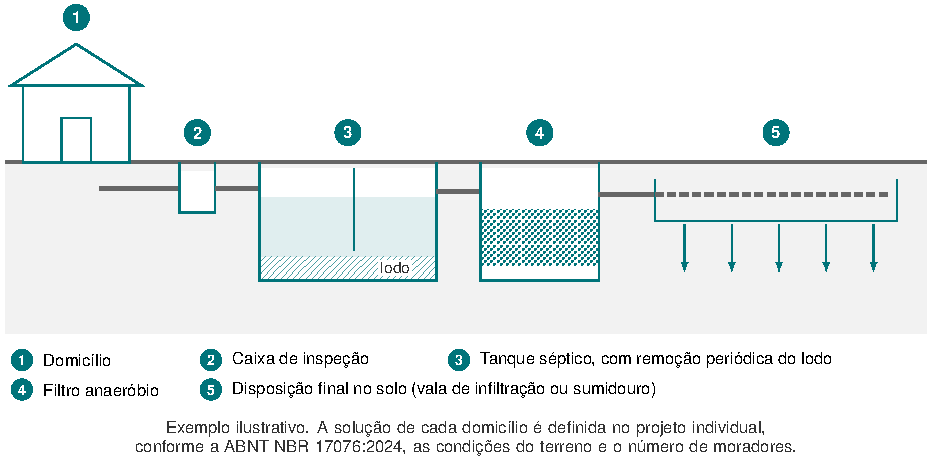
\includegraphics[width=15.78cm]{figuras/f-esquema-esgoto.pdf}
  \fonteMOP{Fonte: IAT (2026), com base em ABNT (2024) e Tonetti et al. (2018). Esquema ilustrativo, sem escala.}
  % Texto alternativo: Esquema em corte com domicílio, caixa de inspeção, tanque séptico, filtro anaeróbio e vala de infiltração.
\end{figure}

A ação contribui para o indicador de pessoas atendidas com, pelo menos, esgotamento sanitário, com cerca de 11,4 mil das 17.800 pessoas previstas; as demais decorrem do esgotamento sanitário em mananciais.

\textbf{Inclui:} a contratação das soluções e das obras civis; o projeto individual de cada domicílio; a instalação conforme a ABNT NBR 17076:2024; a verificação técnica; a orientação do proprietário quanto ao uso e à manutenção; a medição, a comprovação e o pagamento; e a substituição de soluções inadequadas.

\textbf{Não inclui:} redes coletoras nem intervenções no interior das moradias. A manutenção após a entrega, inclusive a limpeza periódica, cabe ao proprietário, conforme a orientação recebida.

\pendencia{Definir o responsável pela coleta e pela destinação do lodo das soluções individuais após a entrega (proprietário, associação, município ou serviço contratado).}

\textbf{Valor previsto:} R\$~32,54 milhões (empréstimo BIRD: R\$~32,54 milhões; contrapartida: R\$~0,00 milhões), conforme a planilha PSH\_CUSTO\_Consolidada.

\phantomsection
\addcontentsline{toc}{subsection}{2. Área de atuação}
\subsection*{2. Área de atuação}

A ação abrange as 83 comunidades atendidas pelos sistemas coletivos de abastecimento de água (Figura~\ref{mapa}). O número de domicílios foi estimado com os dados do Censo 2022 por setor censitário e do CNEFE: dos 5.810 domicílios dessas comunidades, 4.067 (70\%) não dispõem de esgotamento sanitário adequado (IAT, 2026a). Os domicílios atendidos são confirmados individualmente pelo diagnóstico do trabalho técnico-social.

\phantomsection
\addcontentsline{toc}{subsection}{3. Arranjo institucional e partes interessadas}
\subsection*{3. Arranjo institucional e partes interessadas}

O IAT, por meio da DISAR, contrata a empresa, fiscaliza a instalação, valida as medições e efetua o pagamento. A empresa contratada elabora o projeto de cada domicílio e executa a instalação, e o proprietário autoriza a intervenção, acompanha a obra e confirma a execução. A supervisora das obras apoia a fiscalização, e a UGP acompanha a execução.

\begin{itemize}
  \item \textbf{Intervenientes:} empresa contratada; empresa supervisora das obras; prefeituras, no apoio à articulação local;
  \item \textbf{Público envolvido:} proprietários e moradores dos domicílios atendidos.
\end{itemize}

Os beneficiários diretos são os moradores dos 4.067 domicílios sem esgotamento sanitário adequado, cerca de 11,4 mil pessoas. Os beneficiários indiretos são os demais moradores das comunidades e das bacias, em razão da redução da carga de esgoto lançada no solo e nos corpos hídricos.

\phantomsection
\addcontentsline{toc}{subsection}{4. Processo de execução operacional}
\subsection*{4. Processo de execução operacional}

A partir do diagnóstico de cada domicílio, a ação compreende sete etapas (Figura~\ref{raias-3225}). O proprietário participa em dois momentos: autoriza a intervenção na Etapa 1 e confirma a execução na Etapa 6. A evidência de conclusão de cada lote é o relatório técnico aprovado, acompanhado do comprovante de pagamento.

\begin{figure}[H]
  \centering
  \caption{Fluxograma do esgotamento sanitário nas comunidades: entradas, etapas por responsável e saídas}\label{raias-3225}
  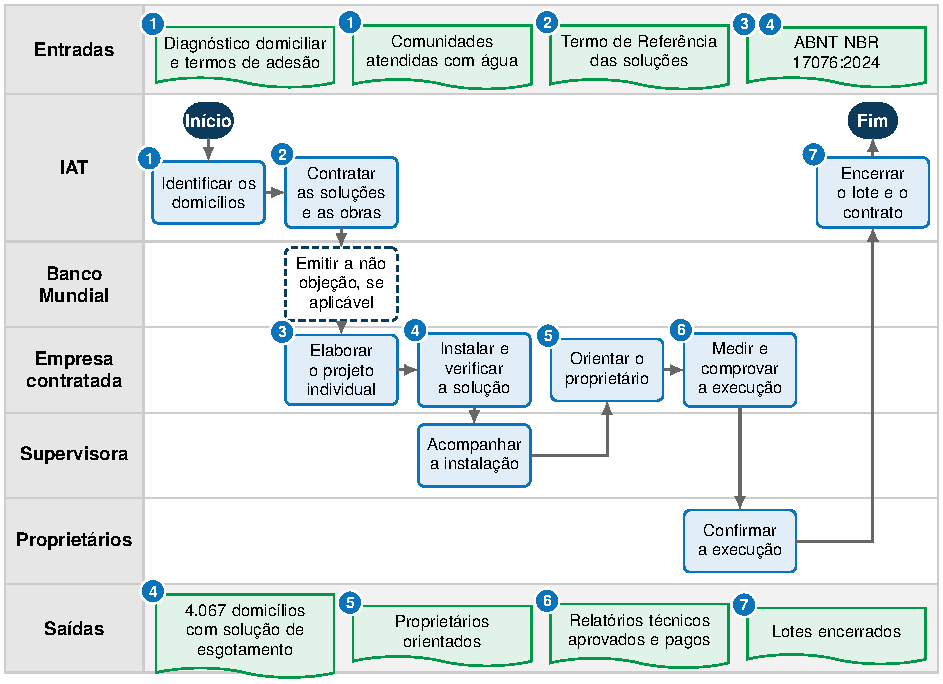
\includegraphics[width=15.96cm]{figuras/g-raias-3225.pdf}
  \fonteMOP{Fonte: IAT (2026).}
  % Texto alternativo: Fluxograma em raias do esgotamento sanitário nas comunidades, com uma raia por instituição, as etapas numeradas na raia do executor, as entradas no topo e as saídas na base.
\end{figure}

\phantomsection
\subsubsection*{4.1 Etapa 1: Identificação dos domicílios}

\textbf{Atividades:} seleção, com base no diagnóstico do trabalho técnico-social, dos domicílios sem esgotamento sanitário adequado; confirmação da adesão e da autorização do proprietário para a intervenção.

\textbf{Entradas:} diagnóstico domiciliar e termos de adesão (trabalho técnico-social).

\textbf{Responsáveis:} IAT (executa e aprova); proprietários (consultados).

\textbf{Produto:} lista de domicílios por comunidade.

\phantomsection
\subsubsection*{4.2 Etapa 2: Contratação das soluções e das obras}

\textbf{Atividades:} elaboração e aprovação do Termo de Referência das soluções descentralizadas e das obras civis de instalação; publicação do edital; licitação; contratação das empresas.

\textbf{Entradas:} lista de domicílios; especificações conforme a ABNT NBR 17076:2024.

\textbf{Responsáveis:} IAT (executa e aprova); UGP e Banco Mundial (consultados, quando houver revisão prévia).

\textbf{Produto:} contrato assinado.

\phantomsection
\subsubsection*{4.3 Etapa 3: Projeto individual por domicílio}

\textbf{Atividades:} elaboração, pela empresa contratada, do projeto de cada domicílio, considerada a topografia do terreno, o número de moradores, a capacidade de infiltração do solo e a solução de tratamento adequada, inclusive o manejo do lodo.

\textbf{Entradas:} contrato; dados do diagnóstico domiciliar.

\textbf{Responsáveis:} empresa contratada (executa); IAT (aprova); proprietário (consultado).

\textbf{Produto:} projeto aprovado.

\phantomsection
\subsubsection*{4.4 Etapa 4: Instalação e verificação técnica}

\textbf{Atividades:} execução das obras civis e instalação dos dispositivos; verificação técnica do funcionamento, da estanqueidade e da garantia. O sistema que atende aos requisitos é validado; o que não atende é corrigido pela empresa e submetido a nova verificação (Figura~\ref{instalacao}).

\begin{figure}[H]
  \centering
  \caption{Projeto, instalação e verificação técnica das soluções individuais}\label{instalacao}
  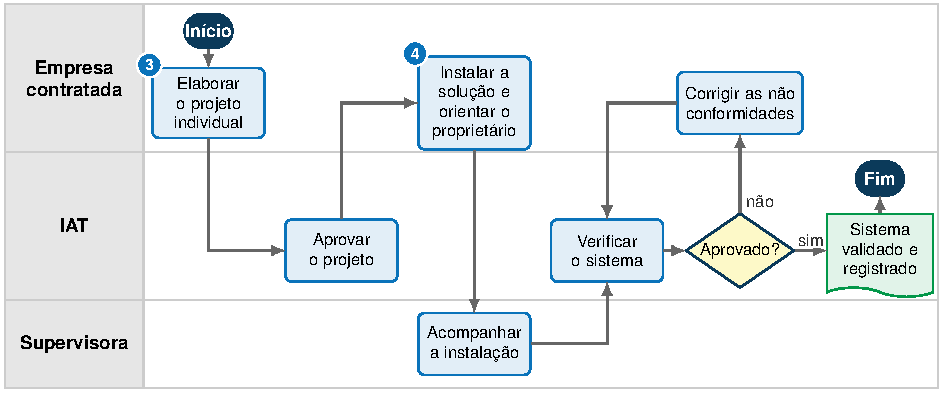
\includegraphics[width=15.96cm]{figuras/f-instalacao.pdf}
  \fonteMOP{Fonte: IAT (2026), com base em IAT (2026b).}
  % Texto alternativo: Fluxograma em raias da empresa contratada, do IAT e da supervisora, do projeto individual à validação do sistema, com a decisão técnica e as correções.
\end{figure}

\textbf{Entradas:} projeto aprovado; autorização do proprietário.

\textbf{Responsáveis:} empresa contratada (executa); supervisora (acompanha); IAT (aprova).

\textbf{Produto:} sistema verificado e validado.

\phantomsection
\subsubsection*{4.5 Etapa 5: Orientação do proprietário}

\textbf{Atividades:} orientação do proprietário, durante a instalação, quanto ao funcionamento do sistema, ao uso adequado, à manutenção preventiva, à limpeza periódica e ao registro da manutenção.

\textbf{Entradas:} sistema em instalação; material de orientação aprovado pelo IAT.

\textbf{Responsáveis:} empresa contratada (executa); IAT (aprova o material); proprietário (participa).

\textbf{Produto:} proprietário orientado, com registro de presença.

\phantomsection
\subsubsection*{4.6 Etapa 6: Medição, comprovação e pagamento}

\textbf{Atividades:} como as soluções são implantadas domicílio a domicílio, o pagamento depende de cadeia de comprovação (Figura~\ref{medicao}). A empresa registra as intervenções em relatórios de medição e reúne as evidências; o proprietário assina o registro de confirmação da execução; o IAT realiza a auditoria documental e as verificações \textit{in loco}; a empresa consolida o relatório de medição final; e o IAT avalia, por amostragem, a qualidade das unidades antes da ordenação da despesa e do pagamento.

\begin{figure}[H]
  \centering
  \caption{Medição, comprovação, verificação e pagamento, por responsável}\label{medicao}
  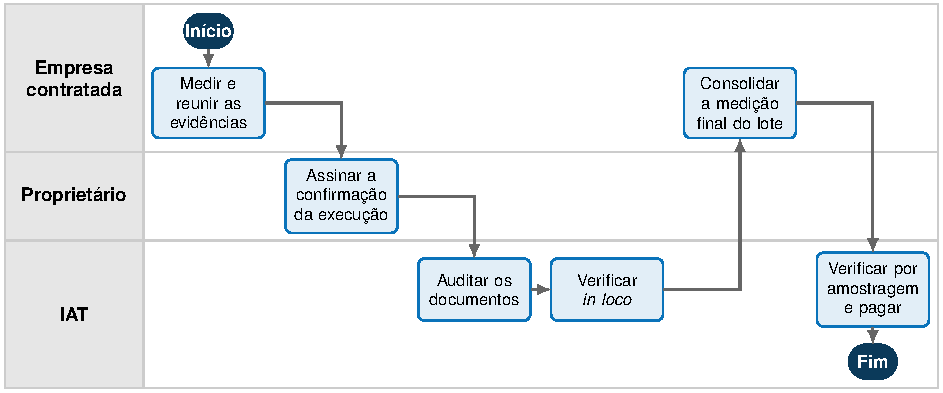
\includegraphics[width=15.96cm]{figuras/f-medicao.pdf}
  \fonteMOP{Fonte: IAT (2026), com base em IAT (2026b).}
  % Texto alternativo: Fluxograma em raias da empresa contratada, do proprietário e do IAT, da medição à amostragem e ao pagamento do lote.
\end{figure}

\textbf{Entradas:} sistemas validados; assinaturas dos proprietários.

\textbf{Responsáveis:} empresa contratada (executa); proprietário (confirma); IAT (verifica, aprova e efetua o pagamento).

\textbf{Produto:} relatório técnico aprovado e comprovante de pagamento, por lote.

\pendencia{Definir o tamanho da amostra da verificação \textit{in loco} e o responsável por cada verificação.}

\phantomsection
\subsubsection*{4.7 Etapa 7: Encerramento}

\textbf{Atividades:} encerramento formal de cada lote e do contrato; consolidação dos resultados para o indicador do componente.

\textbf{Entradas:} relatórios aprovados e pagamentos realizados.

\textbf{Responsáveis:} IAT (executa); UGP (valida).

\textbf{Produto:} lote encerrado.

\phantomsection
\subsubsection*{4.8 Modalidade de execução}

O item de custo é o sistema individual de tratamento de efluentes: 4.067 domicílios a R\$~8.000,00, no total de R\$~32,54 milhões, com recursos do empréstimo do BIRD. A execução ocorre mediante licitação de obras, com o projeto e a instalação no mesmo contrato, conforme o Caderno AQ.

\pendencia{A nota técnica prevê a aquisição centralizada dos materiais pelo IAT, com as obras executadas por empresa contratada; o MOP de março atribuía toda a instalação à empresa. Definir o responsável pela aquisição dos materiais.}

\phantomsection
\addcontentsline{toc}{subsection}{5. Matriz de responsabilidades}
\subsection*{5. Matriz de responsabilidades}

O Quadro~\ref{raci-3225} apresenta o papel de cada parte em cada etapa.

\begin{quadro}[H]
  \caption{Matriz de responsabilidades do esgotamento sanitário nas comunidades}\label{raci-3225}
  \footnotesize\renewcommand{\arraystretch}{1.25}\setlength{\tabcolsep}{3pt}
  \begin{tabular}{>{\raggedright\arraybackslash}p{\dimexpr 0.2536\linewidth-2\tabcolsep\relax}>{\centering\arraybackslash}p{\dimexpr 0.0882\linewidth-2\tabcolsep\relax}>{\centering\arraybackslash}p{\dimexpr 0.0882\linewidth-2\tabcolsep\relax}>{\centering\arraybackslash}p{\dimexpr 0.0882\linewidth-2\tabcolsep\relax}>{\centering\arraybackslash}p{\dimexpr 0.0882\linewidth-2\tabcolsep\relax}>{\centering\arraybackslash}p{\dimexpr 0.0882\linewidth-2\tabcolsep\relax}>{\centering\arraybackslash}p{\dimexpr 0.0882\linewidth-2\tabcolsep\relax}>{\centering\arraybackslash}p{\dimexpr 0.0882\linewidth-2\tabcolsep\relax}>{\centering\arraybackslash}p{\dimexpr 0.1291\linewidth-2\tabcolsep\relax}}
    \rowcolor{azulEscuro}\textcolor{white}{\textbf{Parte}} & \textcolor{white}{\textbf{E1}} & \textcolor{white}{\textbf{E2}} & \textcolor{white}{\textbf{E3}} & \textcolor{white}{\textbf{E4}} & \textcolor{white}{\textbf{E5}} & \textcolor{white}{\textbf{E6}} & \textcolor{white}{\textbf{E7}} & \textcolor{white}{\textbf{Produto final}} \\
    IAT & \raci{R} \raci{A} & \raci{R} \raci{A} & \raci{A} & \raci{A} & \raci{A} & \raci{A} & \raci{R} & \raci{A} \\ \arrayrulecolor{cinza20}\hline
    \rowcolor{cinza5}Empresa contratada & – & – & \raci{R} & \raci{R} & \raci{R} & \raci{R} & \raci{I} & \raci{R} \\ \arrayrulecolor{cinza20}\hline
    Supervisora & – & – & – & \raci{R} & – & \raci{C} & – & – \\ \arrayrulecolor{cinza20}\hline
    \rowcolor{cinza5}Proprietários & \raci{C} & – & \raci{C} & \raci{I} & \raci{R} & \raci{R} & \raci{I} & \raci{I} \\ \arrayrulecolor{cinza20}\hline
    Prefeituras & \raci{I} & – & – & \raci{I} & – & – & \raci{I} & \raci{I} \\ \arrayrulecolor{cinza20}\hline
    \rowcolor{cinza5}UGP & \raci{I} & \raci{C} & \raci{I} & \raci{I} & \raci{I} & \raci{I} & \raci{A} & \raci{I} \\ \arrayrulecolor{cinza20}\hline
    Banco Mundial & – & \raci{C} & – & – & – & – & – & – \\ \noalign{\global\arrayrulewidth=1pt}\arrayrulecolor{azulEscuro}\hline\noalign{\global\arrayrulewidth=0.4pt}
  \end{tabular}
  \fonteMOP{Fonte: IAT (2026).}
  \notaMOP{Nota: E1 a E7 correspondem às Etapas 1 a 7 do item 4. \raci{R} executa (pode haver mais de um); \raci{A} aprova ou valida o produto (um por etapa); \raci{C} é consultado previamente; \raci{I} é informado posteriormente. Produto final: domicílios com solução individual instalada e aprovada.}
\end{quadro}

\phantomsection
\addcontentsline{toc}{subsection}{6. Metas, indicadores e comprovação}
\subsection*{6. Metas, indicadores e comprovação}

O Quadro~\ref{metas-3225} distribui os 4.067 domicílios ao longo do Programa, de forma compatível com o cronograma de implantação dos sistemas de abastecimento.

\begin{quadro}[H]
  \caption{Metas anuais do esgotamento sanitário nas comunidades}\label{metas-3225}
  \footnotesize\renewcommand{\arraystretch}{1.25}\setlength{\tabcolsep}{3pt}
  \begin{tabular}{>{\raggedright\arraybackslash}p{\dimexpr 0.2095\linewidth-2\tabcolsep\relax}>{\raggedright\arraybackslash}p{\dimexpr 0.1268\linewidth-2\tabcolsep\relax}>{\raggedleft\arraybackslash}p{\dimexpr 0.0794\linewidth-2\tabcolsep\relax}>{\raggedleft\arraybackslash}p{\dimexpr 0.0794\linewidth-2\tabcolsep\relax}>{\raggedleft\arraybackslash}p{\dimexpr 0.0794\linewidth-2\tabcolsep\relax}>{\raggedleft\arraybackslash}p{\dimexpr 0.0794\linewidth-2\tabcolsep\relax}>{\raggedleft\arraybackslash}p{\dimexpr 0.0794\linewidth-2\tabcolsep\relax}>{\raggedleft\arraybackslash}p{\dimexpr 0.0794\linewidth-2\tabcolsep\relax}>{\raggedleft\arraybackslash}p{\dimexpr 0.0794\linewidth-2\tabcolsep\relax}>{\raggedleft\arraybackslash}p{\dimexpr 0.1081\linewidth-2\tabcolsep\relax}}
    \rowcolor{azulEscuro}\textcolor{white}{\textbf{Produto}} & \textcolor{white}{\textbf{Unidade}} & \centering\arraybackslash \textcolor{white}{\textbf{Ano 1}} & \centering\arraybackslash \textcolor{white}{\textbf{Ano 2}} & \centering\arraybackslash \textcolor{white}{\textbf{Ano 3}} & \centering\arraybackslash \textcolor{white}{\textbf{Ano 4}} & \centering\arraybackslash \textcolor{white}{\textbf{Ano 5}} & \centering\arraybackslash \textcolor{white}{\textbf{Ano 6}} & \centering\arraybackslash \textcolor{white}{\textbf{Ano 7}} & \centering\arraybackslash \textcolor{white}{\textbf{Total}} \\
    Sistema individual de tratamento de efluentes & domicílios & – & 245 & 477 & 856 & 956 & 956 & 577 & 4.067 \\ \noalign{\global\arrayrulewidth=1pt}\arrayrulecolor{azulEscuro}\hline\noalign{\global\arrayrulewidth=0.4pt}
  \end{tabular}
  \fonteMOP{Fonte: Planilha PSH\_CUSTO\_Consolidada, versão v2408 (PARANÁ, 2026).}
  \notaMOP{Nota: Ano 1 = 2027 e Ano 7 = 2033.}
\end{quadro}

Os indicadores constam do Quadro~\ref{ind-3225}. O indicador do componente corresponde ao número acumulado de domicílios com solução instalada e aprovada multiplicado por 2,8, com desagregação por sexo e para jovens de 15 a 24 anos.

\begin{quadro}[H]
  \caption{Indicadores do esgotamento sanitário nas comunidades}\label{ind-3225}
  \footnotesize\renewcommand{\arraystretch}{1.25}\setlength{\tabcolsep}{3pt}
  \begin{tabular}{>{\raggedright\arraybackslash}p{\dimexpr 0.3165\linewidth-2\tabcolsep\relax}>{\raggedright\arraybackslash}p{\dimexpr 0.1378\linewidth-2\tabcolsep\relax}>{\raggedleft\arraybackslash}p{\dimexpr 0.1102\linewidth-2\tabcolsep\relax}>{\raggedleft\arraybackslash}p{\dimexpr 0.1599\linewidth-2\tabcolsep\relax}>{\raggedright\arraybackslash}p{\dimexpr 0.2756\linewidth-2\tabcolsep\relax}}
    \rowcolor{azulEscuro}\textcolor{white}{\textbf{Indicador}} & \textcolor{white}{\textbf{Unidade}} & \centering\arraybackslash \textcolor{white}{\textbf{Linha de base (2025)}} & \centering\arraybackslash \textcolor{white}{\textbf{Meta}} & \textcolor{white}{\textbf{Frequência e fonte dos dados}} \\
    Domicílios com solução individual instalada e aprovada & domicílios & 0 & 4.067 & Por lote; IAT \\ \arrayrulecolor{cinza20}\hline
    \rowcolor{cinza5}Pessoas atendidas com, pelo menos, esgotamento sanitário (parcela do indicador do componente) & pessoas & 0 & 11.388 & Anual; IAT, com desagregação por sexo e jovens \\ \arrayrulecolor{cinza20}\hline
    Unidades aprovadas na amostragem \textit{in loco} & \% da amostra & – & 100 & Por lote; relatório de amostragem \\ \noalign{\global\arrayrulewidth=1pt}\arrayrulecolor{azulEscuro}\hline\noalign{\global\arrayrulewidth=0.4pt}
  \end{tabular}
  \fonteMOP{Fonte: IAT (2026).}
\end{quadro}

Os critérios de aceite constam do Quadro~\ref{aceite-3225}. A evidência de conclusão de cada lote é o relatório técnico aprovado, acompanhado do comprovante de pagamento.

\begin{quadro}[H]
  \caption{Critérios de aceite e evidências do esgotamento sanitário nas comunidades}\label{aceite-3225}
  \footnotesize\renewcommand{\arraystretch}{1.25}\setlength{\tabcolsep}{5pt}
  \begin{tabular}{>{\raggedright\arraybackslash}p{\dimexpr 0.2150\linewidth-2\tabcolsep\relax}>{\raggedright\arraybackslash}p{\dimexpr 0.3386\linewidth-2\tabcolsep\relax}>{\raggedright\arraybackslash}p{\dimexpr 0.2921\linewidth-2\tabcolsep\relax}>{\raggedright\arraybackslash}p{\dimexpr 0.1543\linewidth-2\tabcolsep\relax}}
    \rowcolor{azulEscuro}\textcolor{white}{\textbf{Produto}} & \textcolor{white}{\textbf{Critério de aceite}} & \textcolor{white}{\textbf{Evidência de comprovação}} & \textcolor{white}{\textbf{Responsável pela validação}} \\
    Projeto individual & Solução adequada ao terreno e ao número de moradores, conforme a ABNT NBR 17076:2024 & Projeto aprovado & IAT \\ \arrayrulecolor{cinza20}\hline
    \rowcolor{cinza5}Sistema instalado & Execução conforme o projeto; teste de estanqueidade aprovado & Relatório de medição; laudo de verificação; registro fotográfico & IAT \\ \arrayrulecolor{cinza20}\hline
    Proprietário orientado & Orientação sobre uso, manutenção e manejo do lodo realizada & Registro de presença & IAT \\ \arrayrulecolor{cinza20}\hline
    \rowcolor{cinza5}Execução confirmada & Execução confirmada pelo proprietário & Assinatura do proprietário & IAT \\ \arrayrulecolor{cinza20}\hline
    Lote aprovado & Auditoria documental, verificação \textit{in loco} e amostragem aprovadas & Relatório técnico aprovado; comprovante de pagamento & IAT \\ \noalign{\global\arrayrulewidth=1pt}\arrayrulecolor{azulEscuro}\hline\noalign{\global\arrayrulewidth=0.4pt}
  \end{tabular}
  \fonteMOP{Fonte: IAT (2026).}
\end{quadro}

\phantomsection
\addcontentsline{toc}{subsection}{7. Gestão de riscos e impactos ambientais e sociais}
\subsection*{7. Gestão de riscos e impactos ambientais e sociais}

Os riscos referem-se à contaminação do solo por instalação inadequada, ao manejo inadequado do lodo, a acidentes durante as obras, à segurança das famílias em razão de valas abertas e à comunicação com os proprietários. As obras ocorrem no interior dos lotes, com autorização do proprietário, sem aquisição de terras (Quadro~\ref{nas-3225}).

\begin{quadro}[H]
  \caption{Aplicação das Normas Ambientais e Sociais ao esgotamento sanitário nas comunidades}\label{nas-3225}
  \footnotesize\renewcommand{\arraystretch}{1.25}\setlength{\tabcolsep}{5pt}
  \begin{tabular}{>{\raggedright\arraybackslash}p{\dimexpr 0.1874\linewidth-2\tabcolsep\relax}>{\raggedright\arraybackslash}p{\dimexpr 0.3716\linewidth-2\tabcolsep\relax}>{\raggedright\arraybackslash}p{\dimexpr 0.4410\linewidth-2\tabcolsep\relax}}
    \rowcolor{azulEscuro}\textcolor{white}{\textbf{NAS}} & \textcolor{white}{\textbf{Aplicação à ação}} & \textcolor{white}{\textbf{Medidas e instrumentos}} \\
    NAS 1 – Avaliação e gestão de riscos & Instalação em cada domicílio & Dimensionamento técnico conforme a ABNT NBR 17076:2024; verificação técnica obrigatória (MGAS) \\ \arrayrulecolor{cinza20}\hline
    \rowcolor{cinza5}NAS 2 – Condições de trabalho & Trabalhadores das empresas contratadas & Uso de EPI; treinamento de segurança; Procedimentos de Gestão de Mão de Obra \\ \arrayrulecolor{cinza20}\hline
    NAS 3 – Eficiência de recursos e prevenção da poluição & Contaminação do solo e da água; lodo e resíduos de obra & Testes de estanqueidade; orientação sobre a limpeza e a destinação do lodo; Plano de Gerenciamento de Resíduos Sólidos \\ \arrayrulecolor{cinza20}\hline
    \rowcolor{cinza5}NAS 4 – Saúde e segurança da comunidade & Valas abertas nos lotes, com circulação de crianças e animais & Sinalização, isolamento e proteção das valas; execução em prazo reduzido em cada domicílio \\ \arrayrulecolor{cinza20}\hline
    NAS 10 – Engajamento das partes interessadas & Proprietários e moradores & Autorização prévia; reuniões com linguagem acessível; Mecanismo de Queixas e Reclamações (PEPI e MQR) \\ \noalign{\global\arrayrulewidth=1pt}\arrayrulecolor{azulEscuro}\hline\noalign{\global\arrayrulewidth=0.4pt}
  \end{tabular}
  \fonteMOP{Fonte: IAT (2026), com base nos instrumentos do Caderno AS.}
  \notaMOP{Nota: a NAS 5 não se aplica, por não haver aquisição de terras; as NAS 6, 7 e 8 são verificadas na triagem das comunidades.}
\end{quadro}

\phantomsection
\addcontentsline{toc}{subsection}{8. Cronograma}
\subsection*{8. Cronograma}

A contratação ocorre em 2028, e os projetos, as instalações, a orientação e as medições, de 2028 a 2033, conforme a planilha de custos: 245 domicílios em 2028, 477 em 2029, 856 em 2030, 956 em 2031 e em 2032 e 577 em 2033 (Figura~\ref{crono-3225}).

\begin{figure}[H]
  \centering
  \caption{Cronograma das etapas e das entregas do esgotamento sanitário nas comunidades}\label{crono-3225}
  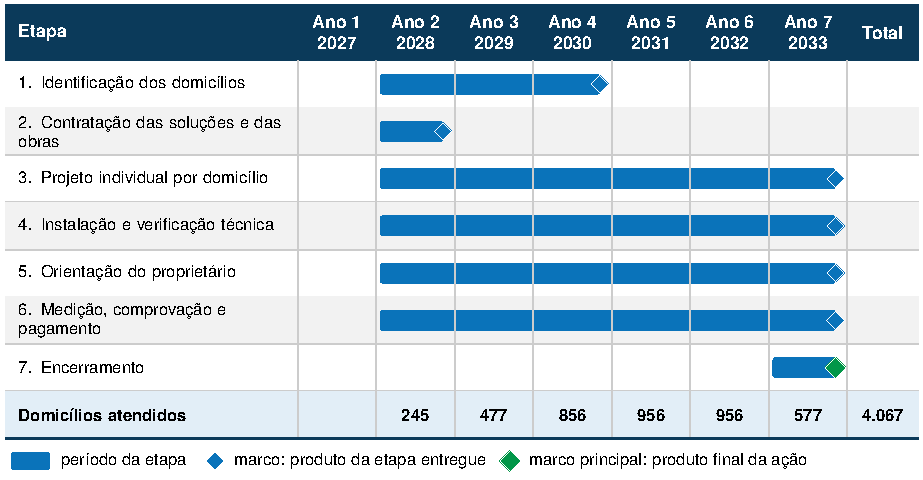
\includegraphics[width=15.64cm]{figuras/g-crono-3225.pdf}
  \fonteMOP{Fonte: IAT (2026), com quantidades da planilha PSH\_CUSTO\_Consolidada (PARANÁ, 2026).}
  % Texto alternativo: Cronograma anual de 2027 a 2033 com as etapas e as quantidades a entregar do esgotamento sanitário nas comunidades.
\end{figure}

\phantomsection
\addcontentsline{toc}{subsection}{9. Interfaces e dependências}
\subsection*{9. Interfaces e dependências}

A ação recebe do trabalho técnico-social o diagnóstico domiciliar e os termos de adesão; da implantação dos sistemas de abastecimento, as comunidades atendidas e o cronograma das obras; e da supervisão das obras, o acompanhamento das instalações. Fornece o número de pessoas atendidas para o indicador do componente e reduz a carga de esgoto lançada no solo e nos corpos hídricos (Figura~\ref{interf-3225}).

\begin{figure}[H]
  \centering
  \caption{Interfaces e dependências do esgotamento sanitário nas comunidades}\label{interf-3225}
  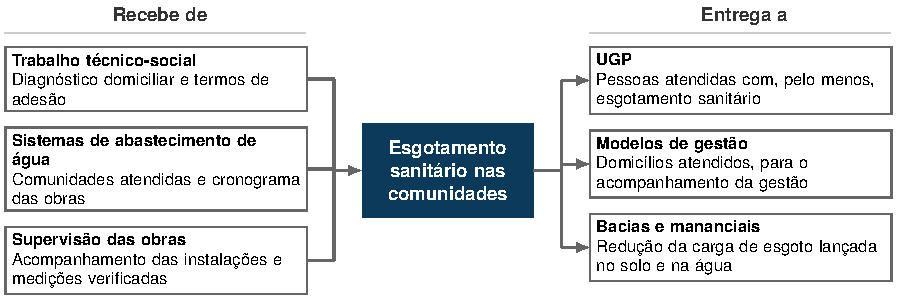
\includegraphics[width=15.30cm]{figuras/g-interf-3225.pdf}
  \fonteMOP{Fonte: IAT (2026).}
  % Texto alternativo: Diagrama das interfaces do esgotamento sanitário nas comunidades: insumos recebidos de outras partes do Programa e produtos entregues a elas.
\end{figure}

\phantomsection
\addcontentsline{toc}{subsection}{10. Documentos complementares}
\subsection*{10. Documentos complementares}

\begin{itemize}
  \item ABNT NBR 17076:2024 (ABNT, 2024);
  \item Termo de Referência e edital das soluções descentralizadas e das obras civis (a elaborar);
  \item Modelo de autorização e de confirmação da execução pelo proprietário (a elaborar);
  \item Material de orientação do proprietário sobre uso, manutenção e manejo do lodo (a elaborar);
  \item Tonetti et al. (2018), referência para a seleção das soluções;
  \item Caderno AQ e Caderno AS.
\end{itemize}
